\chapter{Field Content of the Standard Model}
\label{sec:Field}

The \ac{SM} of particle physics is a quantum field theory that combines the concept of classic field theory with quantum mechanics and special relativity. Different elementary particles can be described as the excited states of distinct quantum fields, characterized by masses and various quantum numbers. A summary of the known elementary particles and their properties is given in Figure~\ref{fig:Field}.

\begin{figure}[tbh!]
 \begin{center}
 \begin{tabular}{c}
 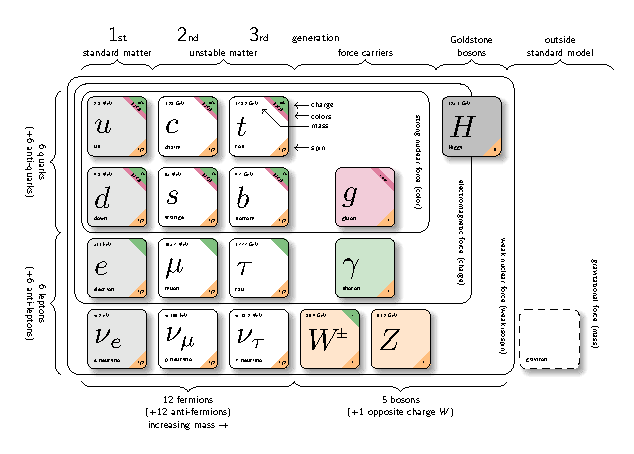
\includegraphics[width=\textwidth]{figures/Part1/Field/SM}
 \end{tabular}
 \caption{The field content of the \ac{SM}, including all known elementary particles. The three generations of fermions are shown in the first three columns. The gauge bosons that mediate the fundamental interactions are shown in fourth and fifth columns. The sixth column shows the recently discovered Higgs boson. The hypothetical graviton that mediates gravitational force is also shown, which is outside of realm of the \ac{SM}.~\cite{tikz:SM}}
 \label{fig:Field}
 \end{center}
\end{figure}

The effects described by special relativity apply to all elementary particles. This requires the the theory to be invariant under Lorentz transformations, which contain rotations and Lorentz boosts of the coordinate systems. The behaviors of elementary particles under such transformations, characterized by their spin quantum numbers, divide particles into two groups. Those with half integer spins are known as ``fermions'', which are described in \ref{sec:Fermion} in details. Particles with integer spins are known as ``bosons'', which are described in \autoref{sec:Boson} in details. 

\section{Fermion}
\label{sec:Fermion}

Named after Italian physicist Enrico Fermi, fermions follow Fermi-Dirac statistics and obey the Pauli exclusion principle, which prohibits two or more fermions with the same quantum number from simultaneously occupying the same quantum state. The matter existed in the universe is made up of spin-$\frac{1}{2}$ fermions represented by ``spinors'' under Lorentz transformations. For example, the free Lagrangian that encodes full information of a spinor field can be expressed as,

\begin{equation}
\label{eq:lefthand}
\mathcal{L}=i\psi_{L}^{\dagger}\sigma^{\mu}\partial_{\mu}\psi_{L}
\end{equation}
or
\begin{equation}
\label{eq:righthand}
\mathcal{L}=i\psi_{R}^{\dagger}\bar{\sigma}^{\mu}\partial_{\mu}\psi_{R},
\end{equation}

where $\sigma^{\mu}$ is the 2$\times$2 Pauli matrix. The spinors in Equation~\ref{eq:lefthand}-\ref{eq:righthand} are known as Weyl spinors, which correspond to a two-dimensional irreducible representation of the Lorentz group. Weyl spinors can be classified into left handed spinros $\psi_{L}$ or right handed spinors $\psi_{R}$ depending on the orientation of their spin relative to their momentum. More formally, $\psi_{L}$ and $\psi_{R}$ correspond to the ($\frac{1}{2}$,0) and (0,$\frac{1}{2}$) representation of the Lorentz group~\cite{zee:group}.

In addition to Lorentz invariance, the free Lagrangians should also be invariant under parity transformation. For Weyl spinors, however, this symmetry is clearly violated as right handed spinors transform into left hand spinors under parity, and vice versa. To describe elementary fermions, the two irreducible representations must be stacked together, forming a four-dimensional reducible representation ($\frac{1}{2}$,0) $\bigoplus$ (0,$\frac{1}{2}$),

\begin{equation}
\label{eq:leftandright}
\mathcal{L}=i\psi_{L}^{\dagger}\sigma^{\mu}\partial_{\mu}\psi_{L}+i\psi_{R}^{\dagger}\bar{\sigma}^{\mu}\partial_{\mu}\psi_{R}.
\end{equation}

It is also possible to introduce additional Lorentz- and parity-invariant terms $m(\psi_{L}^{\dagger}\psi_{R}+\psi_{R}^{\dagger}\psi_{L})$ to Equation~\ref{eq:leftandright},

\begin{equation}
\label{eq:DiracLag}
\mathcal{L}_{Dirac}=i\psi_{L}^{\dagger}\sigma^{\mu}\partial_{\mu}\psi_{L}+i\psi_{R}^{\dagger}\bar{\sigma}^{\mu}\partial_{\mu}\psi_{R}+m(\psi_{L}^{\dagger}\psi_{R}+\psi_{R}^{\dagger}\psi_{L}),
\end{equation}

where $m$ corresponds to the physical mass of the fermions. Equation~\ref{eq:DiracLag} is known as the Dirac Lagrangian. Using the Euler-Lagrange equation that is based on the principle of least action,

\begin{equation}
\frac{\partial\mathcal{L}}{\partial\psi}-\partial_{\mu}\frac{\partial\mathcal{L}}{\partial(\partial_{\mu}\mathcal{L})}=0,
\end{equation}

the equation of motion for the Dirac Lagrangian can be written as,

\begin{equation}
\label{eq:Dirac1}
i\sigma^{\mu}\partial_{\mu}\psi_{L}=m\psi_{R}
\end{equation}
\begin{equation}
\label{eq:Dirac2}
i\bar{\sigma}^{\mu}\partial_{\mu}\psi_{R}=m\psi_{L}
\end{equation}

Defining the four-dimensional Dirac spinor as $\psi=\begin{psmallmatrix}\psi_{L}\\\psi_{R}\end{psmallmatrix}$ and the 4$\times$4 Dirac matrix as $\gamma^{\mu}=\begin{psmallmatrix}0&\bar{\sigma}^{\mu}\\\sigma^{\mu}&0\end{psmallmatrix}$, Equation~\ref{eq:Dirac1}-\ref{eq:Dirac2} can be rewritten as,

\begin{equation}
\label{eq:Dirac}
i\gamma^{\mu}\partial_{\mu}\psi-m\psi=0,
\end{equation}

which is the famed Dirac equation first derived by British physicist Paul Dirac. Ironically, Dirac arrived at this equation with a simple goal of finding an equation with only one power of derivative, and was puzzled by the negative-energy solutions to his equation. It was later understood these negative-energy solutions correspond to anti-particles that have the same mass but opposite signs of all quantum numbers. The existence of such particles was first confirmed by American physicist C. D. Anderson in 1932, who used cloud chamber to produce to first photographic evidence of positron, which is shown in Figure~\ref{fig:Positron}.

\begin{figure}[tbh!]
 \begin{center}
 \begin{tabular}{c}
 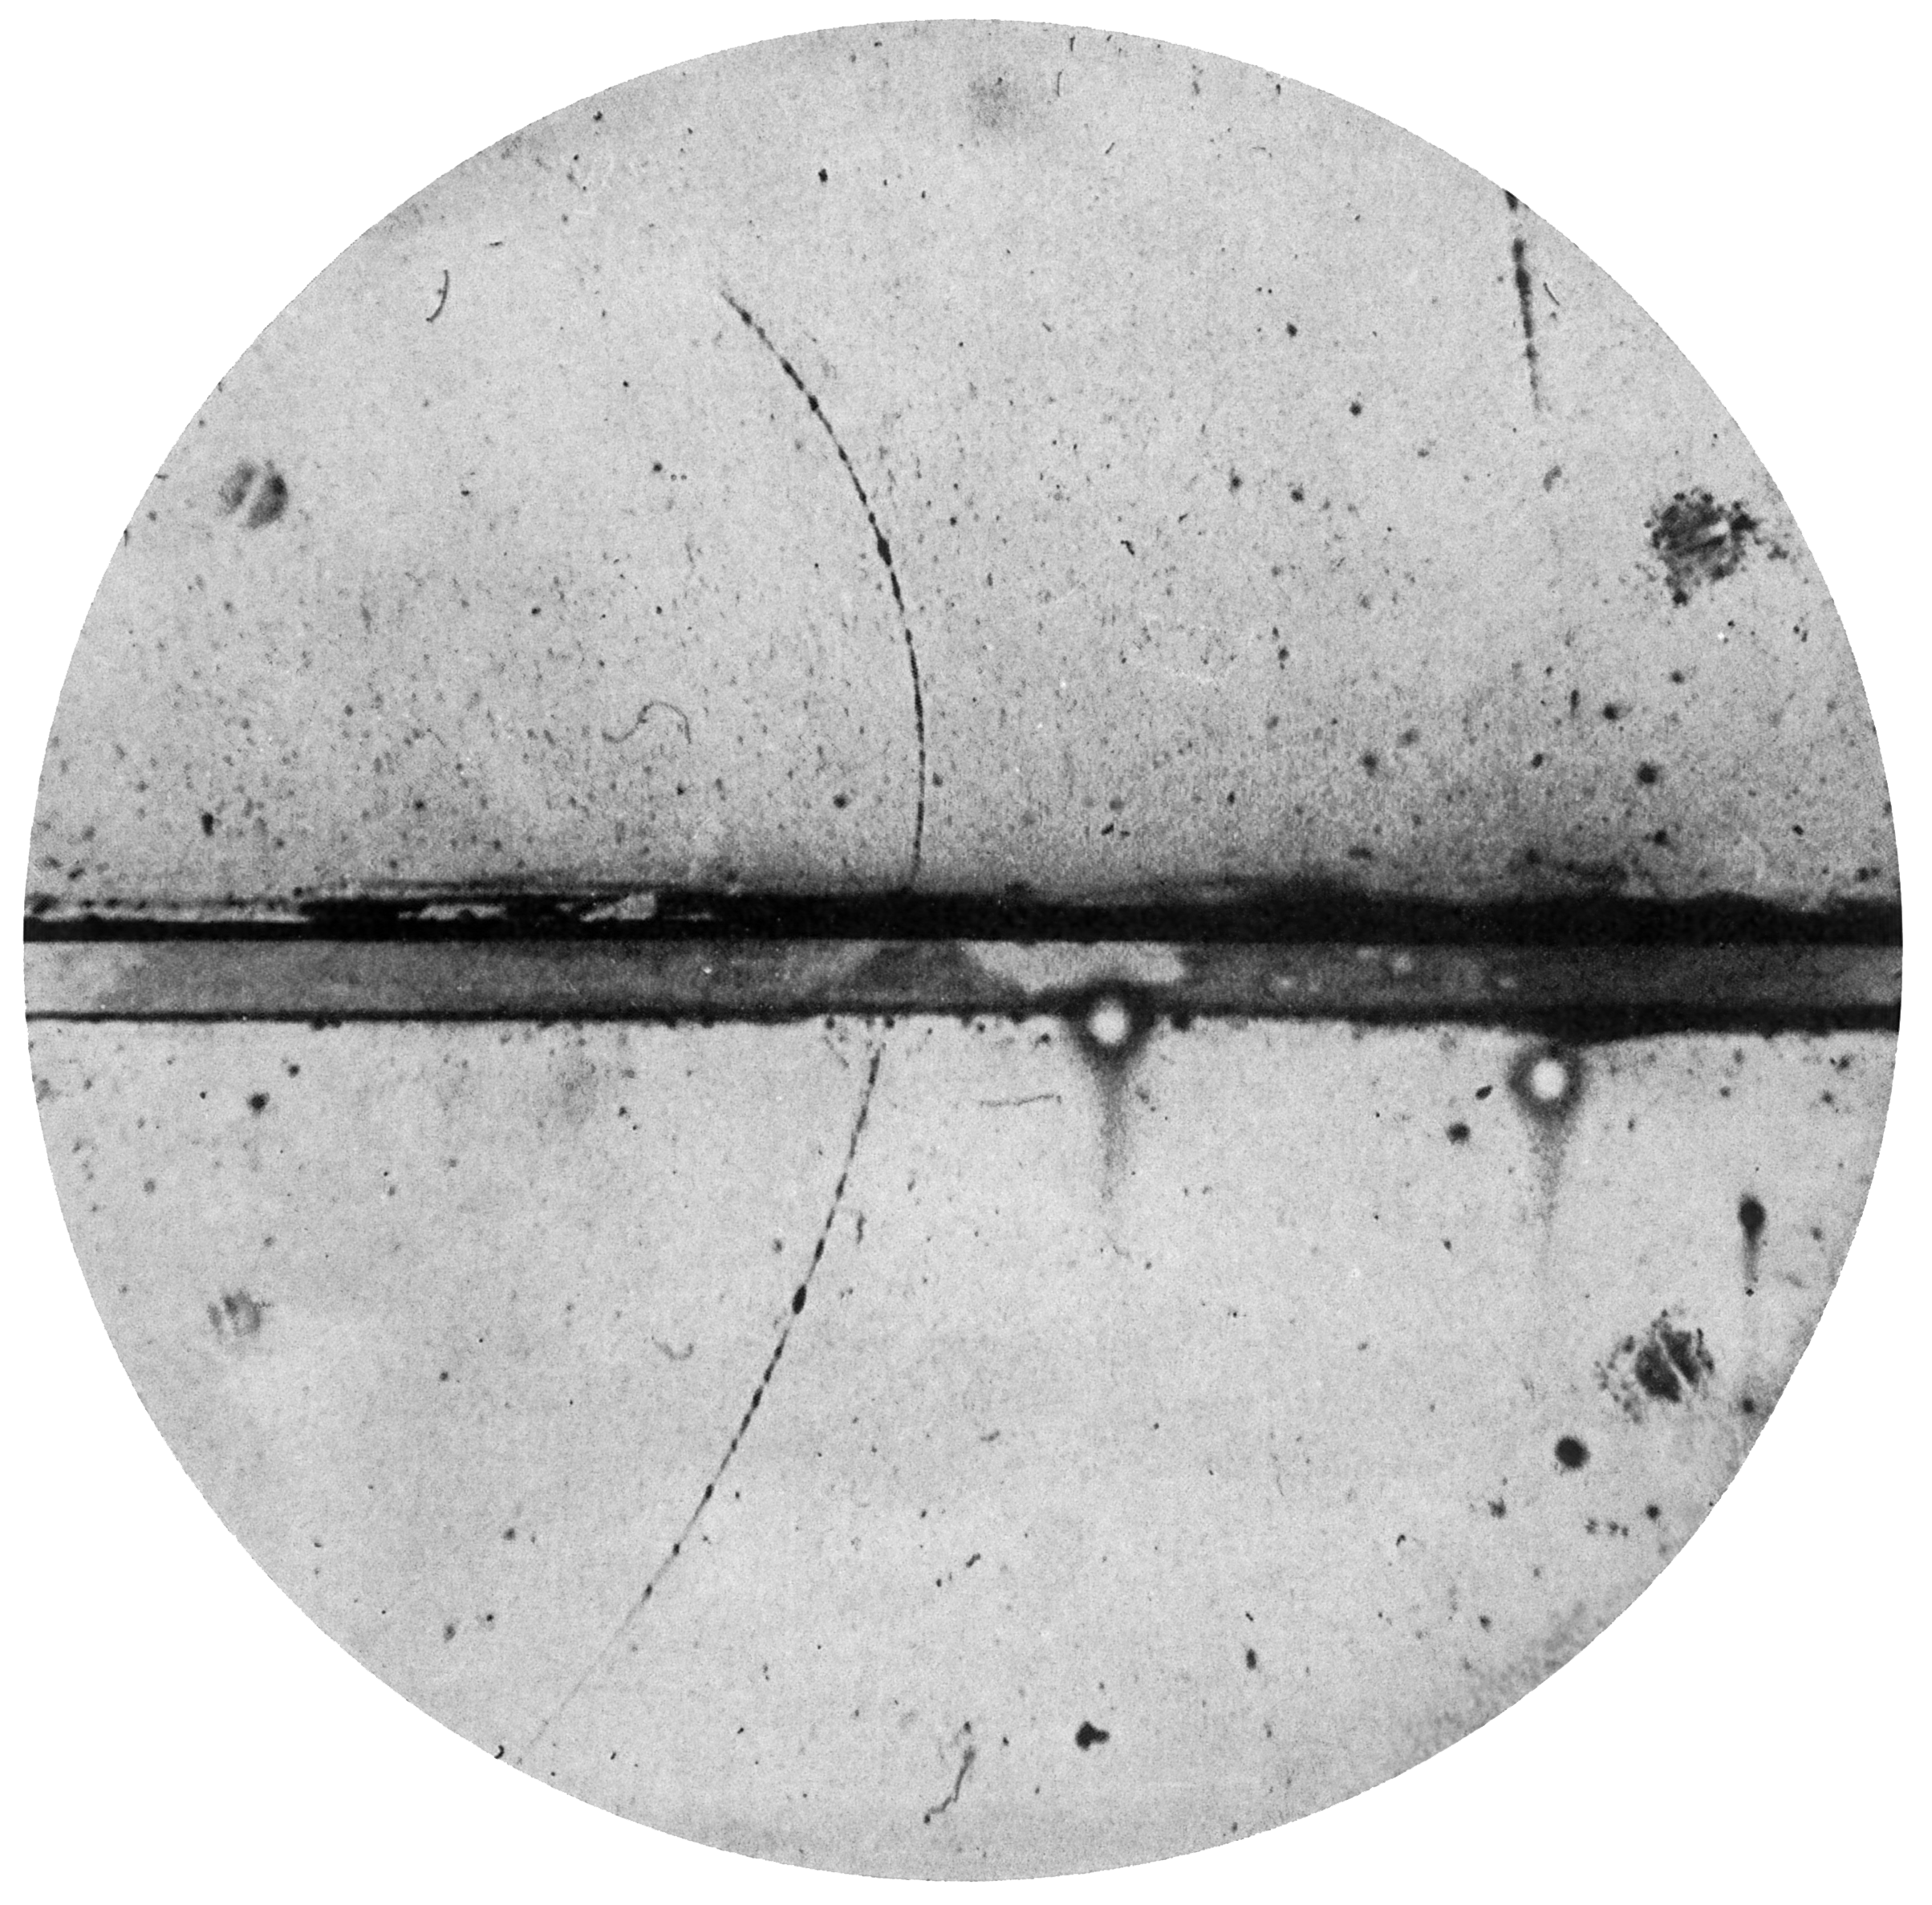
\includegraphics[width=0.55\textwidth]{figures/Part1/Field/Positron}
 \end{tabular}
 \caption{The field content of the \ac{SM}, including all known elementary particles. The three generations of fermions are shown in the first three columns. The gauge bosons that mediate the fundamental interactions are shown in fourth and fifth columns. The sixth column shows the recently discovered Higgs boson. The hypothetical graviton that mediates gravitational force is also shown, which is outside of realm of the \ac{SM}.~\cite{tikz:SM}}
 \label{fig:Positron}
 \end{center}
\end{figure}

Elementary fermions are classified into two groups, quarks and leptons. Quarks are affected by all fundamental forces. 

\begin{figure}[tbh!]
 \begin{center}
 \begin{tabular}{c}
 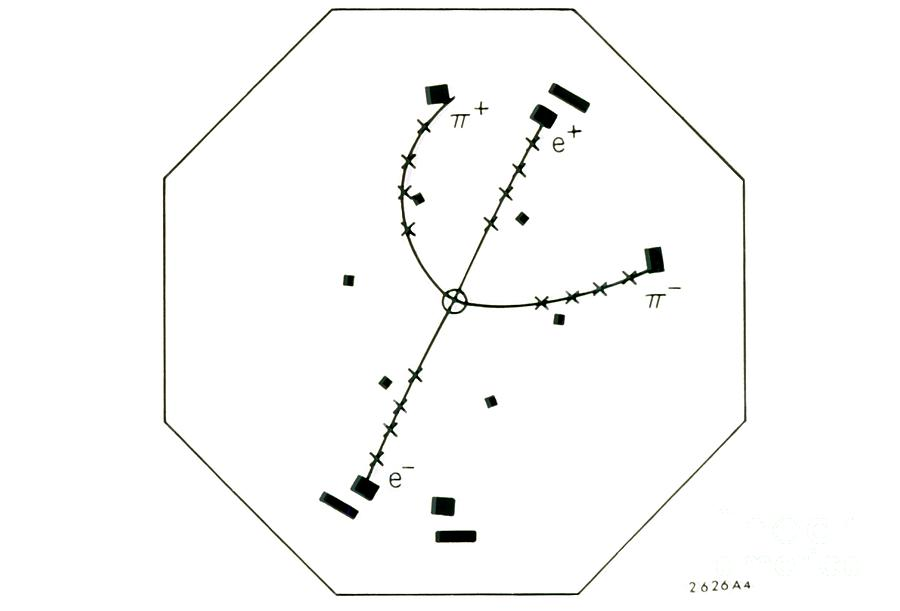
\includegraphics[width=0.7\textwidth]{figures/Part1/Field/J}
 \end{tabular}
 \caption{The field content of the \ac{SM}, including all known elementary particles. The three generations of fermions are shown in the first three columns. The gauge bosons that mediate the fundamental interactions are shown in fourth and fifth columns. The sixth column shows the recently discovered Higgs boson. The hypothetical graviton that mediates gravitational force is also shown, which is outside of realm of the \ac{SM}.~\cite{tikz:SM}}
 \label{fig:JPsi}
 \end{center}
\end{figure}

\section{Boson}
\label{sec:Boson}